

% \section{Factors Affecting MAS Performance}
\section{哪些因素会影响 MAS 性能？}
\label{sec:analysis}

% \update{
基于\cref{sec:analysis_setup}提出的分析框架，我们通过实证分析研究不同因素如何影响 MAS 相对于 SAS 的性能。具体而言，我们关注三个研究问题：\textbf{RQ1：} \cref{sec:five_axis_framework}所刻画的任务结构与验证协议如何影响 MAS 性能（\cref{sec:subtask_structure}）；\textbf{RQ2：}编排器的初始化如何影响 MAS 性能（\cref{sec:reasoning_meta_agent}）；\textbf{RQ3：}子智能体能力如何影响 MAS 性能（\cref{sec:reasoning_sub_agent}）。
% Together, these analyses yield clear observations and takeaways that clarify when and why MAS provide advantages over SAS.
% }

在所有分析中，我们都使用所提出的 \ourframework 训练编排器来生成 MAS，同时固定所有子智能体。为排除异构子智能体能力造成的混杂影响，我们将候选子智能体限制为 \textsc{CoTAgent}，并排除其他子智能体（例如 \texttt{DeepResearchAgent}）。对于 SAS，我们使用相同的 \textsc{CoTAgent}，不进行任何额外训练。我们将 \masness 设为\textit{高}，使编排器可以生成包含灵活数量 \textsc{CoTAgent} 的 MAS。
我们使用 \ourbenchmark 在受控维度下生成的合成训练数据来训练编排器，并在留出的测试实例上评估 SAS 与 MAS。更多细节见\cref{ap:training_setup}。

\subsection{不同评估维度如何影响 MAS？}
\label{sec:subtask_structure}
% \zixuan{TODO: add connection}
%We hypothesize that MAS performs better on certain sub-task properties than others. 
% Thanks to \ourbenchmark, we can now systematically test how different axes of sub-task structure affect performance. 
不同维度代表不同的任务结构与验证协议，刻画不同的推理和协作需求。我们研究它们如何影响 MAS 性能。
% We vary the sub-agent between GPT-OSS-120b (low) (G-120b (low)) \cite{openai2025gptoss120bgptoss20bmodel} and Qwen-2.5-7b-instr (Q-7b) \cite{qwen2.5}, while initializing the orchestrator with Q-7b for orchestrator training. 
% \zixuan{Others are moved to appendix}
{
% We conduct several analyses to investigate these effects, including MAS vs. SAS comparisons, separate vs. combined training, \robustness without adversarial data, and complexity generaliztion. Those analysis are detailed in \cref{ap:discuss_control}.
我们重点考察它们对\textit{最终结果}的影响，并在\cref{ap:discuss_control}中给出生成的 MAS、复杂度泛化等补充分析。}
% \zixuan{complexity generaliztion moved to Appendix}
% \shafiq{for Qwen ... and GPT ...}.
% Figures \ref{fig:sub_task_sub_agent} and \ref{fig:robustness} show the results on the first 4 axes and the robustness axis, respectively.

 
\begin{center}
\vspace{-0.5\baselineskip}
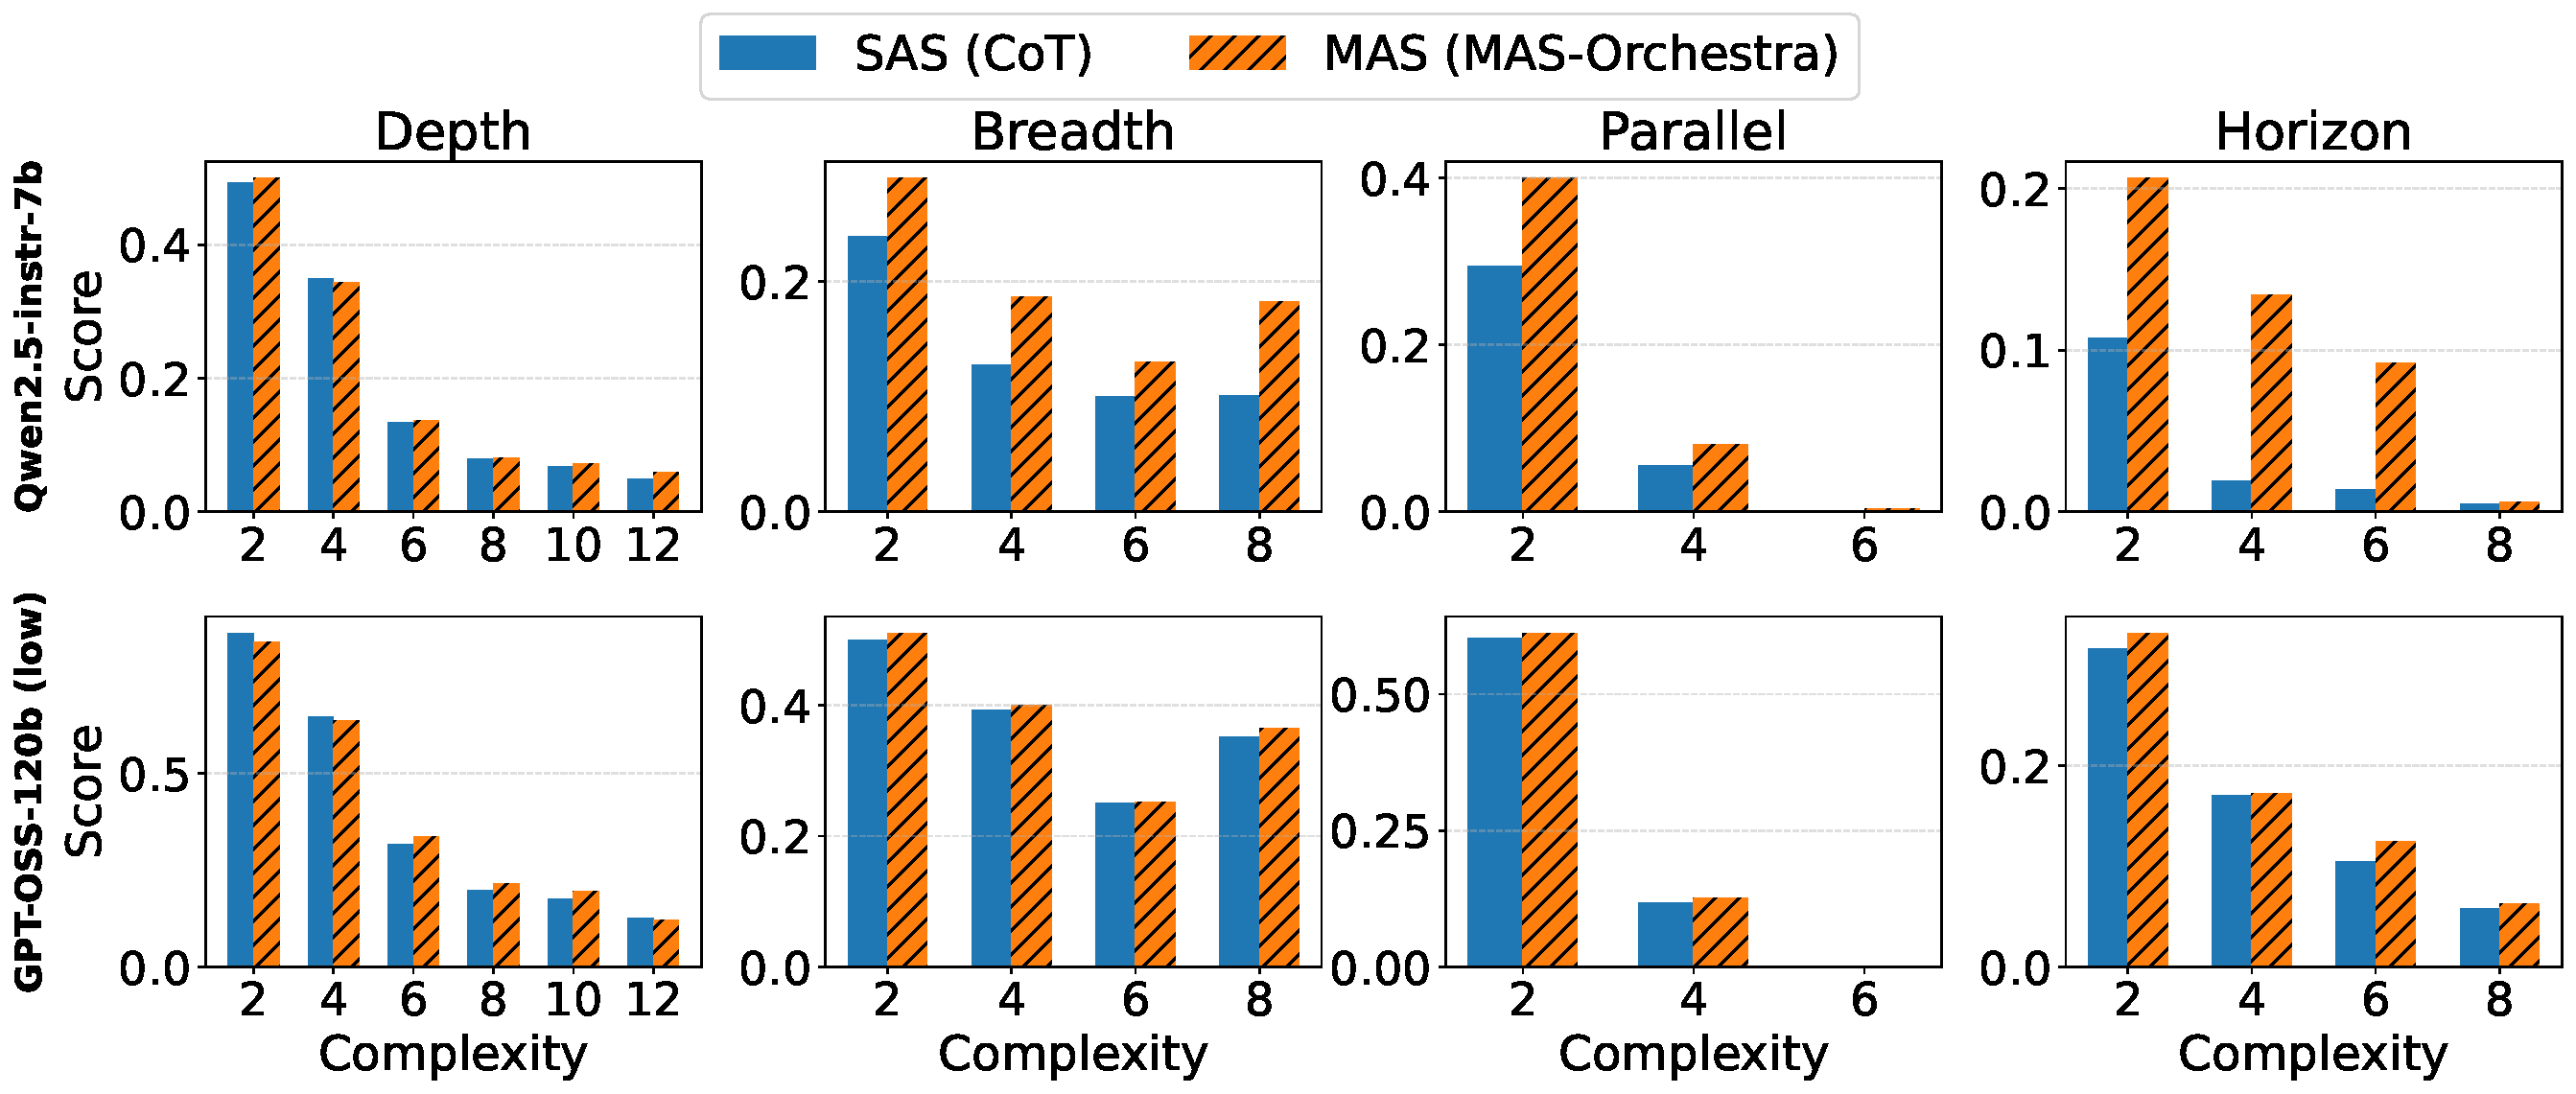
\includegraphics[width=\columnwidth]{figs/sub_task_sub_agent.pdf}
\vspace{-12pt}
\captionof{figure}{\small SAS 与 MAS 在各维度上的 \avgat{8} 准确率。编排器使用 Qwen-2.5-7B-Instr（\qwen）初始化，子智能体分别采用 \qwen 和 GPT-OSS-120B（\ossonetwentylow）。}
% \austin{This caption is separated from the figure}
% {(accuracy) for SAS and MAS} across different axes with Qwen-2.5-7b-instr (\qwen) \cite{qwen2.5} as initialization for orchestrator training, \qwen and GPT-OSS-120b (\ossonetwentylow) \cite{openai2025gptoss120bgptoss20bmodel} as sub-agent. 
% \zixuan{parallel 6 is always 0, perhas can remove} 
\label{fig:sub_task_sub_agent}
\end{center}

\textbf{当子智能体“较弱”（\qwen）时，除 \depth 维度外，MAS（\ourframework）在大多数子任务结构上都优于 SAS}（\cref{fig:sub_task_sub_agent}上图）。
这一结果不难理解：当子任务高度相互依赖且必须严格按顺序解决时，单条顺序 CoT 可以减少不必要的分支与协作开销。在这种情况下，MAS 引入的额外编排收益有限，因而削弱了其相对于 SAS 的优势。
% which limits the advantage of MAS. 

\textbf{当子智能体“较强”（\ossonetwentylow）时，MAS 在 \depth、\horizon、\breadth 和 \myparallel 上的性能收益都会减小}（\cref{fig:sub_task_sub_agent}下图）。这表明，随着子智能体能力增强，MAS 的收益会下降。在这种情况下，协作成本与智能体间的误差传播可能抵消 MAS 的潜在收益，最终无法带来净提升。


\textbf{在数据投毒下，MAS 始终表现出更强的 \robustness，而 SAS 在这一对抗环境中的准确率几乎降至零}（\cref{fig:robustness}）。
这表明 MAS 天生更能抵御投毒输入，因为冗余、交叉验证以及结构化的智能体间交互提供了单智能体系统所不具备的保护机制。

为了说明这一行为，\cref{tab:sas_mas_example}给出了一个代表性示例。
% \footnote{We will release all examples upon acceptance.} 
我们观察到 SAS 可能非常不可靠：它往往不验证注释，而是直接接受其中的信息，最终得出错误结论。相比之下，\ourframework 能显式分解问题，并将不同的（彼此冲突的）子任务分配给不同子智能体。在该示例中，MAS 引入了一个\emph{最终答案}智能体，由它充当\emph{仲裁者}；该智能体识别对抗信号，并通过提示词设计提供恰当线索或纠正性指导，从而缓解其影响。对于不同子任务意图可能具有误导性的数据投毒场景，这种结构化编排提供了更鲁棒的处理方式。通过在子智能体之间分配职责并引入仲裁步骤，MAS 能够实现比单智能体方法更可靠的推理。

% \begin{takeaway} 
\textbf{MAS 在\textit{子智能体能力边界}上最有效。}综合上述观察可知，当底层子智能体具备一定能力、但尚不足以独自可靠地内化复杂任务结构时，MAS 相对于 SAS 能带来明显收益。在这种情况下（例如任务结构并非纯顺序式，或任务包含潜在的对抗性子任务），显式分解、编排与仲裁有助于释放并利用潜在推理能力。
% \zixuan{this is takeaway}
% (1) The sub-task is not sequential (depth); (2) the agent is required to keep track of the intermediate results; (3) SAS has not internalized the underlying sub-task structure; (4) The task contains potential adversarial sub-tasks.
% \end{takeaway}


\subsection{RLM 是否是更好的编排器初始化？}
\label{sec:reasoning_meta_agent}

% Having established the effect of sub-task structure, we next 
我们考察用作编排器的底层 LLM 所发挥的作用。为了隔离编排器的贡献，我们固定子智能体，并在指令微调 LLM 与推理语言模型（RLM）之间改变编排器。

\begin{center}
\vspace{-0.5\baselineskip}
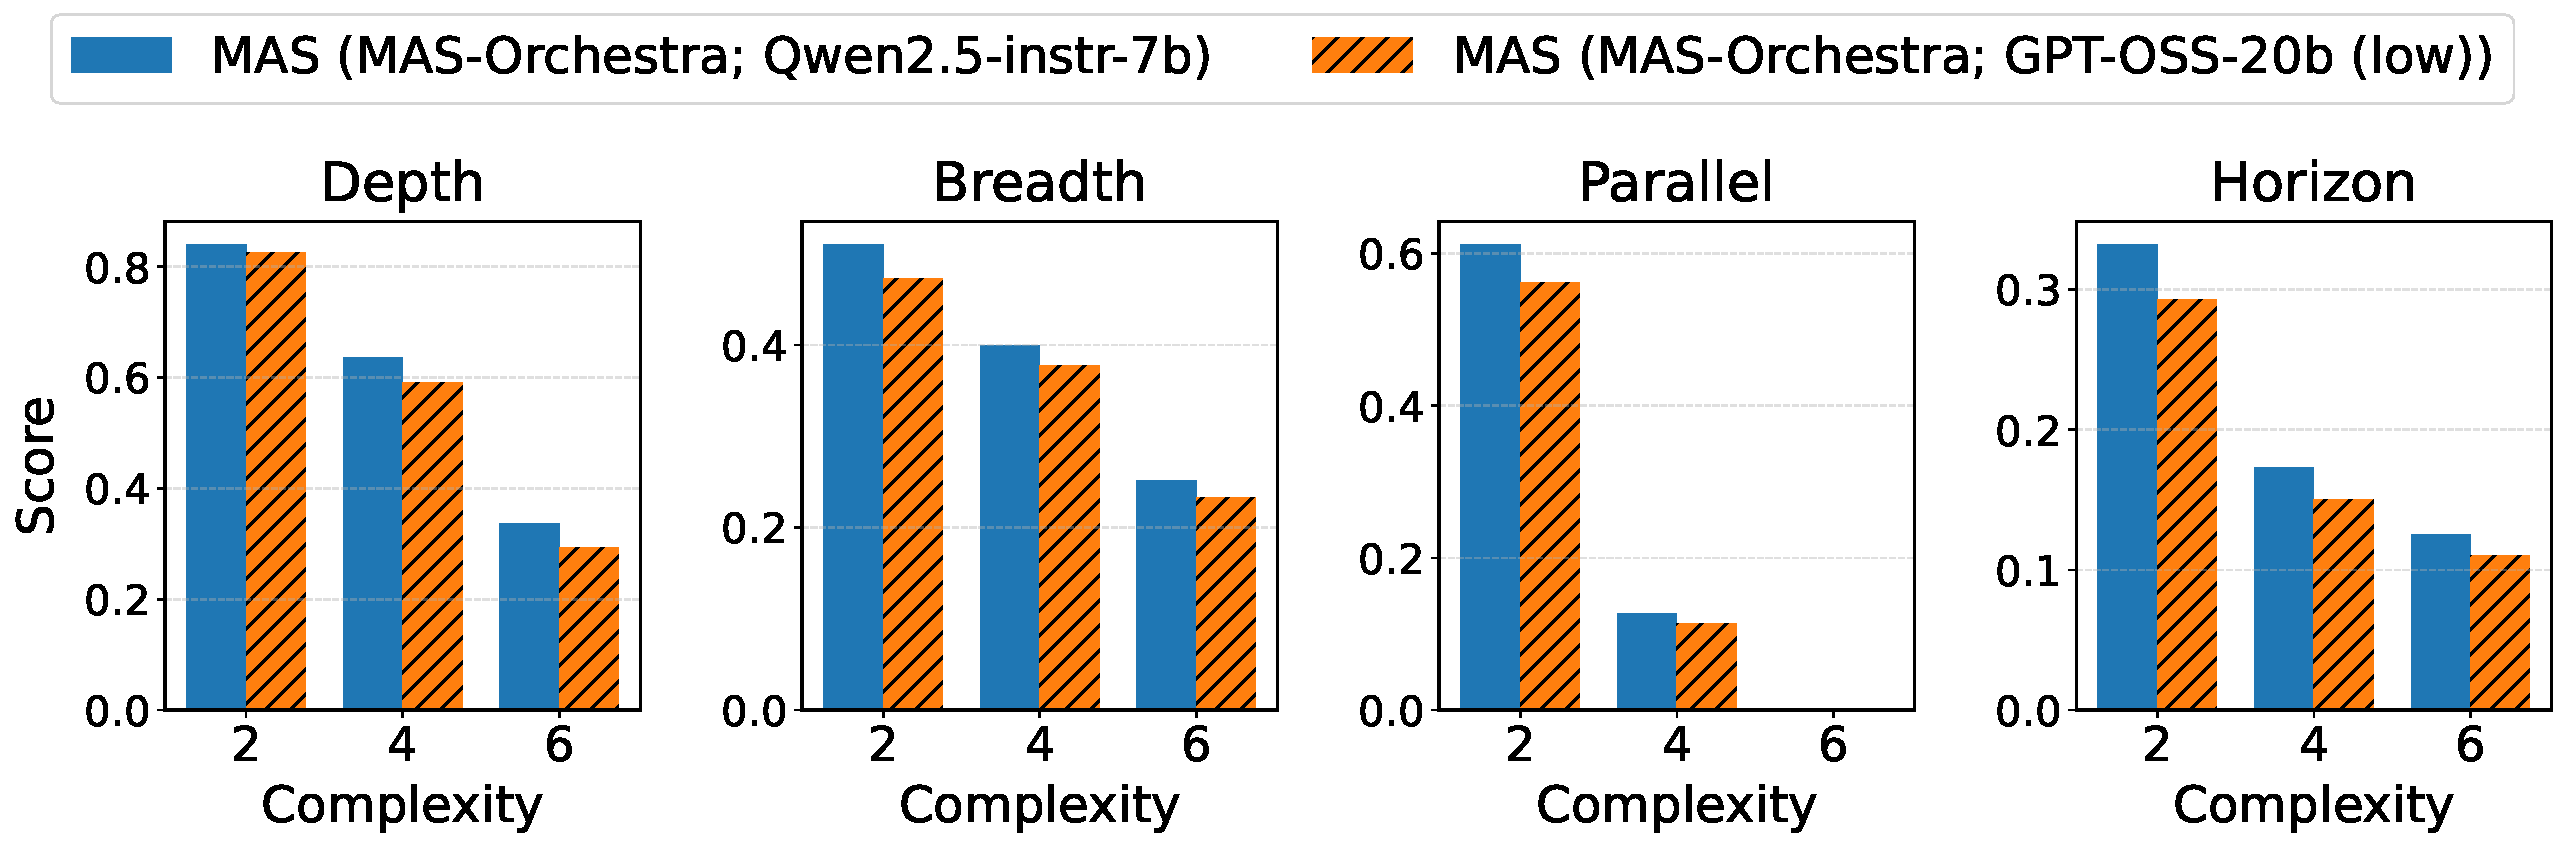
\includegraphics[width=\columnwidth]{figs/meta_ilm_vs_rlm.pdf}
\vspace{-\baselineskip}
\captionof{figure}{\small 以 LLM 和 RLM 作为编排器时的 \avgat{8} 准确率对比。编排器分别使用 \qwen 和 \osstwenty 初始化，子智能体采用 \ossonetwentylow（更多 RLM 的结果见\cref{fig:deepseek}）。}
\label{fig:meta_ilm_vs_rlm}
\end{center}

\textbf{采用指令微调 LLM 初始化的编排器优于采用 RLM 初始化的编排器}（\cref{fig:meta_ilm_vs_rlm}）。
这一结果起初令人意外，因为已有研究表明 RLM 在许多推理任务上优于 LLM。\textit{然而，先前工作并未系统研究 RLM 作为编排器时的有效性。}

为此，我们分析了 \ourframework 所提出 MAS 中的\textit{智能体统计信息}。如\cref{fig:7b_120b_vs_20b_120b_depth4}所示，基于 RLM 的编排器倾向于生成简单得多的 MAS，有时只包含一个子智能体；随着训练收敛，这种模式会逐渐占据主导。相比之下，指令微调 LLM 编排器在任务委派上更加灵活，三个智能体的配置最终成为主流。进一步查看\cref{tab:rlm_example}中的代表性示例可以发现，RLM 倾向于\textit{先自行解决任务，再将任务仅委派给一个简单子智能体，即使该子智能体（\ossonetwentylow）解决任务的能力更强}。这种行为说明 RLM 更重视直接解题而非任务委派，这可能反映了其端到端训练目标。相比之下，指令微调 LLM 针对指令遵循和协调进行优化，因此更符合有效编排所需的结构化控制。

% This behavior suggests that RLMs prioritize direct task solving over delegation. We speculate that this arises because RLMs are primarily trained for end-to-end problem solving, whereas instruction-tuned LLMs are trained to follow instructions and are therefore better suited for orchestrator roles. More broadly, these observations indicate that effective orchestration prioritizes task decomposition, delegation, and
% coordination over directly solving sub-tasks. Current RLM training objectives
% emphasize end-to-end problem solving rather than structural control, making
% them misaligned with the requirements of orchestration.

% We extract the MAS and shows some typical examples in \cref{ap:rlm_orchestrator}. We found the the RLM tends to solve the task itself, rather then following the instruction to do orchestation: it \zixuan{solve, and say it is easy...}


% We speculate that this is because RLM is highly trained for direct task solving rather than task delegation, whereas LLMs are trained to follow instruction and perform better in orchestrator roles.

% The above observations suggest that effective orchestration prioritizes task decomposition, delegation, and
% coordination over directly solving sub-tasks. Current RLM training objectives
% emphasize end-to-end problem solving rather than structural control, making
% them misaligned with the requirements of orchestration.
% \end{takeaway}

% \zixuan{need example...}

% 1. Qwen2.5-7b,  GPT-OSS-20b-low, Qwen2.5-deepseek

% weaker sub-agent and stronger sub-agent



\subsection{子智能体的推理强度如何影响 MAS？}
% \austin{Affect [x]?}
\label{sec:reasoning_sub_agent}
% \zixuan{we may remove sub-section 4.4, as it is "negative fidnings? but robustness we are still consistenly better"}
% We have shown that a stronger underlying LLM for sub-agent can reduce the benefit of MAS
% (\cref{sec:subtask_structure}) and that instruction-tuned LLMs serve as more
% effective orchestrators. Building on these findings, 
我们固定编排器为 \qwen，并令子智能体使用 \ossonetwenty 的 \{低、中、高\}推理强度，以考察子智能体推理能力的影响。需要指出的是，编排器始终使用处于\textit{低}推理强度的子智能体进行训练（默认最大长度为 512 个词元），再使用更高推理强度的子智能体评估训练后的编排器。这一设置使我们能够判断 MAS 能否跨不同推理强度泛化。
% \cref{fig:reasoning_effort} shows the results.
% we fix the orchestrator to be \qwen and employ stronger sub-agents by using \ossonetwentymid and \ossonetwentyhigh.

\begin{center}
\vspace{-0.5\baselineskip}
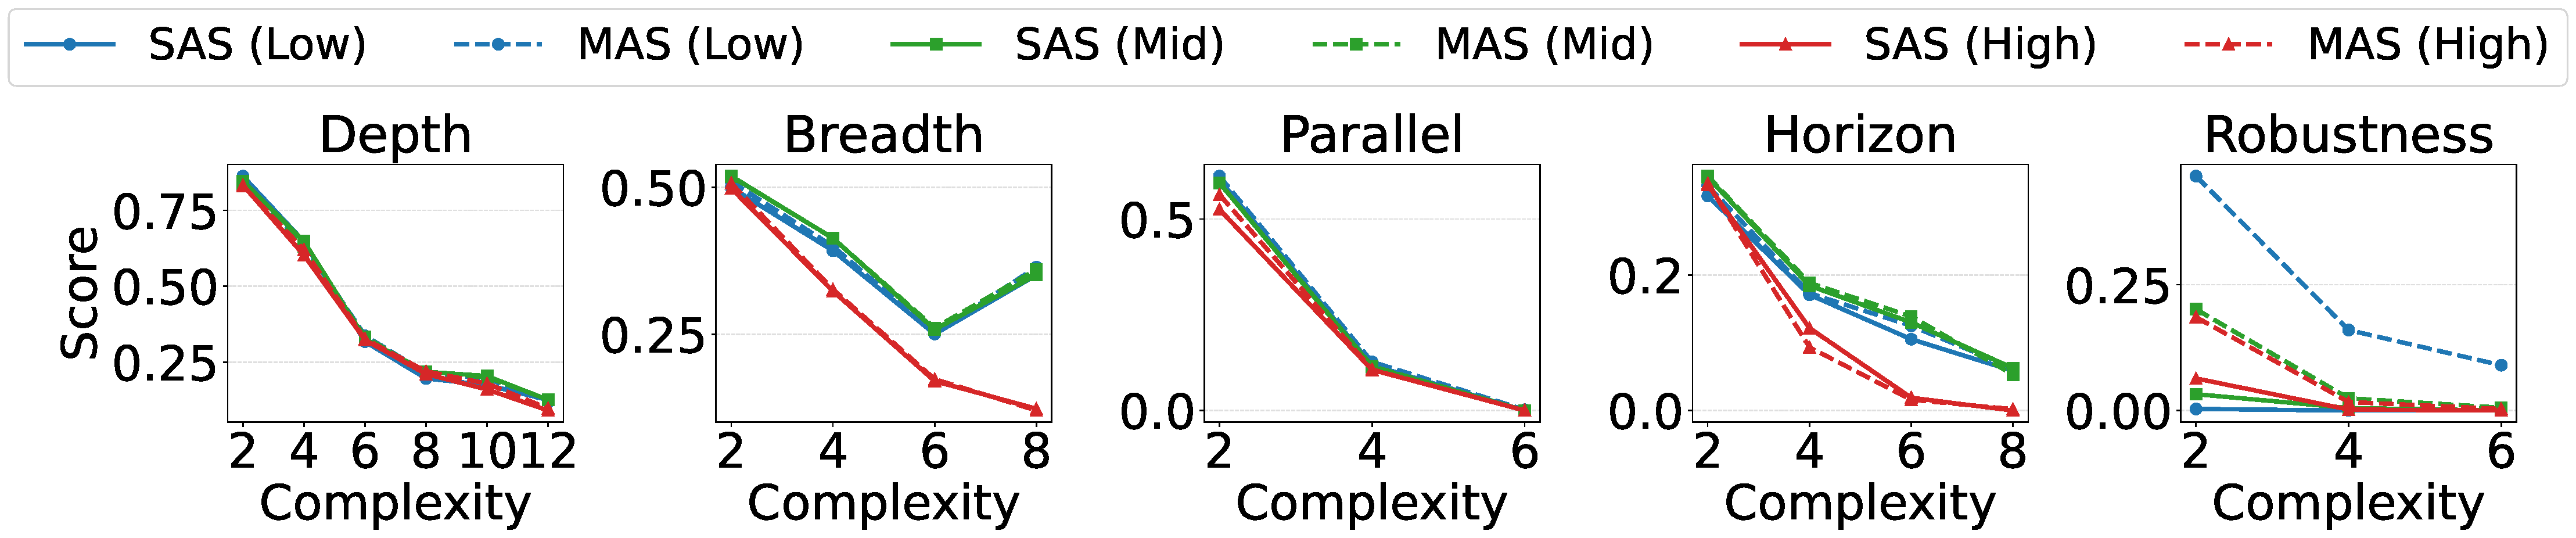
\includegraphics[width=\columnwidth]{figs/reasoning_effort.pdf}
\vspace{-\baselineskip}
\captionof{figure}{\small 不同推理强度下的 \avgat{8} 准确率对比，其中编排器为 \qwen，子智能体为 \ossonetwenty。}
% \vspace{-\baselineskip}
\label{fig:reasoning_effort}
\end{center}

% We fi and various different sub-agent

% 1. Qwen2.5-7b and GPT-OSS-120b \zixuan{same as above}


\textbf{在更高推理强度下，MAS 同样无法免于超出最大上下文长度限制}（\cref{fig:reasoning_effort}）。我们观察到，对 MAS 和 SAS 而言，提高推理强度都未能比低推理强度带来更好性能。进一步检查生成样本后发现，更高推理强度会显著增加超出默认最大上下文长度的概率。一旦达到上下文上限，两个系统的性能都会下降。这并不意外，因为我们的模型只在低推理强度下训练。因此，要有效处理更长的推理轨迹，需要针对上下文管理与长度控制进行显式训练。

% We consistently observe that
% increasing reasoning effort makes it easier to hit the context limit, especially as task complexity grows.
% When the context limit is reached, both MAS and SAS experience performance
% degradation. This is understandable, as our models are trained only with low reasoning
% effort. Effectively handling longer reasoning traces therefore requires
% explicit training for context management and length control.

% Notably, MAS are not immune to this effect. 
% (a default response length of 512 tokens was used)

%\begin{discussion} 
\textbf{上下文长度更长时，MAS 可在高推理强度下提升 \robustness。}
% \zixuan{"training" is not very accurate} 
我们进一步将最大上下文长度提高到极限（\ossonetwenty 子智能体为 12 万词元）。如\cref{fig:max_length}所示，我们观察到了与\cref{fig:reasoning_effort}和\cref{fig:sub_task_sub_agent}一致的趋势：MAS 在 \robustness 上最为有效。这说明，即使子智能体以高推理强度运行，MAS 提供的鲁棒性收益仍然存在，并非有限上下文或推理截断造成的假象。
% In contrast, increasing reasoning effort alone does not address context management challenges, which likely require dedicated training.

% Taken together, these observations suggest that adversarial robustness is the primary regime in which MAS provide consistent benefits, including under high reasoning effort.
% Above observations show that adversarial robustness remains the primary regime where MAS provide consistent
% gains, including when sub-agents operate with high reasoning effort. 
% In
% contrast, effective context management likely requires dedicated training
% rather than increased reasoning effort alone. 
